% intro/intro.tex

\QuickQuizChapter{chp:Introduction}{Introduction}

Parallel programming has earned a reputation as one of the most
difficult areas a hacker can tackle.
Papers and textbooks warn of the perils of deadlock, livelock,
race conditions, non-determinism, Amdahl's-Law limits to scaling,
and excessive realtime latencies.
And these perils are quite real; we authors have accumulated uncounted
% 2009:
%	19 for Paul E. McKenney
years of experience dealing with them, and all of the emotional scars,
grey hairs, and hair loss that go with such experiences.

However, new technologies that are difficult to use at introduction
invariably become easier over time.
For example, the once-rare ability to drive a car is now
commonplace in many countries.
This dramatic change came about for two basic reasons: (1)~cars became
cheaper and more readily available, so that more people had the
opportunity to learn to drive, and (2)~cars became easier to operate
due to automatic transmissions, automatic chokes, automatic starters,
greatly improved reliability,
and a host of other technological improvements.

The same is true of a host of other technologies, including computers.
It is no longer necessary to operate a keypunch in order to program.
Spreadsheets allow most non-programmers to get results from their computers
that would have required a team of specialists a few decades ago.
Perhaps the most compelling example is web-surfing and content creation,
which since the early 2000s has been easily done by
untrained, uneducated people using various now-commonplace
social-networking tools.
As recently as 1968, such content creation was a far-out research
project~\cite{DouglasEngelbart1968}, described at
the time as
``like a UFO landing on the White House lawn''\cite{ScottGriffen2000}.
% http://www.ibiblio.org/pioneers/engelbart.html
% http://www.histech.rwth-aachen.de/www/quellen/engelbart/ahi62index.html

Therefore, if you wish to argue that parallel programming will remain
as difficult as it is currently perceived by many to be, it is you
who bears the burden of proof, keeping in mind the many centuries of
counter-examples in a variety of fields of endeavor.

\section{Historic Parallel Programming Difficulties}
\label{sec:intro:Historic Parallel Programming Difficulties}

As indicated by its title, this book takes a different approach.
Rather than complain about the difficulty of parallel programming,
it instead examines the reasons why parallel programming is
difficult, and then works to help the reader to overcome these
difficulties.
As will be seen, these difficulties have fallen into several categories,
including:

\begin{enumerate}
\item	The historic high cost and relative rarity of parallel systems.
\item	The typical researcher's and practitioner's lack of experience
	with parallel systems.
\item	The paucity of publicly accessible parallel code.
\item	The lack of a widely understood engineering discipline of
	parallel programming.
\item	The high overhead of communication relative to that of processing,
	even in tightly coupled shared-memory computers.
\end{enumerate}

Many of these historic difficulties are well on the way to being overcome.
First, over the past few decades, the cost of parallel systems
has decreased from many multiples of that of a house to a fraction of
that of a bicycle, courtesy of Moore's Law.
Papers calling out the advantages of multicore CPUs were published
as early as 1996~\cite{Olukotun96}.
IBM introduced simultaneous multi-threading
into its high-end POWER family in 2000, and multicore in 2001.
Intel introduced hyperthreading into its commodity Pentium line in
November 2000, and both AMD and Intel introduced
dual-core CPUs in 2005.
Sun followed with the multicore/multi-threaded Niagara in late 2005.
In fact, by 2008, it was becoming difficult
to find a single-CPU desktop system, with single-core CPUs being
relegated to netbooks and embedded devices.
By 2012, even smartphones were starting to sport multiple CPUs.

Second, the advent of low-cost and readily available multicore systems
means that the once-rare experience of parallel programming is
now available to almost all researchers and practitioners.
In fact, parallel systems are now well within the budget of students
and hobbyists.
We can therefore expect greatly increased levels of invention and
innovation surrounding parallel systems, and that increased familiarity
will over time make the once prohibitively expensive field of parallel
programming much more friendly and commonplace.

Third, in the 20\textsuperscript{th} century, large systems of
highly parallel software were almost always closely guarded proprietary
secrets.
In happy contrast, the 21\textsuperscript{st} century has seen numerous
open-source (and thus publicly available) parallel software projects,
including the Linux kernel~\cite{Torvalds2.6kernel},
database systems~\cite{PostgreSQL2008,MySQL2008},
and message-passing systems~\cite{OpenMPI2008,BOINC2008}.
This book will draw primarily from the Linux kernel, but will
provide much material suitable for user-level applications.

Fourth, even though the large-scale parallel-programming projects of
the 1980s and 1990s were almost all proprietary projects, these
projects have seeded the community with a cadre of developers who
understand the engineering discipline required to develop production-quality
parallel code.
A major purpose of this book is to present this engineering discipline.

Unfortunately, the fifth difficulty, the high cost of communication
relative to that of processing, remains largely in force.
Although this difficulty has been receiving increasing attention during
the new millennium, according to Stephen Hawking,
the finite speed of light and the atomic
nature of matter is likely to limit progress in this
area~\cite{BryanGardiner2007,GordonMoore03a}.
Fortunately, this difficulty has been in force since the late 1980s,
so that the aforementioned engineering discipline has evolved practical
and effective strategies for handling it.
In addition, hardware designers are increasingly aware of these issues,
so perhaps future hardware will be more friendly to parallel software
as discussed in Section~\ref{sec:cpu:Hardware Free Lunch?}.

\QuickQuiz{}
	Come on now!!!
	Parallel programming has been known to be exceedingly
	hard for many decades.
	You seem to be hinting that it is not so hard.
	What sort of game are you playing?
\QuickQuizAnswer{
	If you really believe that parallel programming is exceedingly
	hard, then you should have a ready answer to the question
	``Why is parallel programming hard?''
	One could list any number of reasons, ranging from deadlocks to
	race conditions to testing coverage, but the real answer is that
	{\em it is not really all that hard}.
	After all, if parallel programming was really so horribly difficult,
	how could a large number of open-source projects, ranging from Apache
	to MySQL to the Linux kernel, have managed to master it?

	A better question might be: ''Why is parallel programming {\em
	perceived} to be so difficult?''
	To see the answer, let's go back to the year 1991.
	Paul McKenney was walking across the parking lot to Sequent's
	benchmarking center carrying six dual-80486 Sequent Symmetry CPU
	boards, when he suddenly realized that he was carrying several
	times the price of the house he had just purchased.\footnote{
		Yes, this sudden realization {\em did} cause him to walk quite
		a bit more carefully.
		Why do you ask?}
	This high cost of parallel systems meant that
	parallel programming was restricted to a privileged few who
	worked for an employer who either manufactured or could afford to
	purchase machines costing upwards of \$100,000 --- in 1991 dollars US.

	In contrast, in 2006, Paul finds himself typing these words on a
	dual-core x86 laptop.
	Unlike the dual-80486 CPU boards, this laptop also contains
	2GB of main memory, a 60GB disk drive, a display, Ethernet,
	USB ports, wireless, and Bluetooth.
	And the laptop is more than an order of magnitude cheaper than
	even one of those dual-80486 CPU boards, even before taking inflation
	into account.

	Parallel systems have truly arrived.
	They are no longer the sole domain of a privileged few, but something
	available to almost everyone.

	The earlier restricted availability of parallel hardware is
	the \emph{real} reason that parallel programming is considered
	so difficult.
	After all, it is quite difficult to learn to program even the simplest
	machine if you have no access to it.
	Since the age of rare and expensive parallel machines is for the most
	part behind us, the age during which
	parallel programming is perceived to be mind-crushingly difficult is
	coming to a close.\footnote{
		Parallel programming is in some ways more difficult than
		sequential programming, for example, parallel validation
		is more difficult.
		But no longer mind-crushingly difficult.}
} \QuickQuizEnd

However, even though parallel programming might not be as hard as
is commonly advertised, it is often more work than is sequential
programming.

\QuickQuiz{}
	How could parallel programming \emph{ever} be as easy
	as sequential programming?
\QuickQuizAnswer{
	It depends on the programming environment.
	SQL~\cite{DIS9075SQL92} is an underappreciated success
	story, as it permits programmers who know nothing about parallelism
	to keep a large parallel system productively busy.
	We can expect more variations on this theme as parallel
	computers continue to become cheaper and more readily available.
	For example, one possible contender in the scientific and
	technical computing arena is MATLAB*P,
	which is an attempt to automatically parallelize common
	matrix operations.

	Finally, on Linux and UNIX systems, consider the following
	shell command:

	{\small \tt get\_input | grep "interesting" | sort}

	This shell pipeline runs the \co{get_input}, \co{grep},
	and \co{sort} processes in parallel.
	There, that wasn't so hard, now was it?

	In short, parallel programming is just as easy as sequential
	programming---at least in those environments that hide the parallelism
	from the user!
} \QuickQuizEnd

It therefore makes sense to consider alternatives to parallel programming.
However, it is not possible to reasonably consider parallel-programming
alternatives without understanding parallel-programming goals.
This topic is addressed in the next section.

\section{Parallel Programming Goals}
\label{sec:intro:Parallel Programming Goals}

The three major goals of parallel programming (over and above those
of sequential programming) are as follows:

\begin{enumerate}
\item	Performance.
\item	Productivity.
\item	Generality.
\end{enumerate}

\QuickQuiz{}
	Oh, really???
	What about correctness, maintainability, robustness, and so on?
\QuickQuizAnswer{
	These are important goals, but they are just as important for
	sequential programs as they are for parallel programs.
	Therefore, important though they are, they do not belong on
	a list specific to parallel programming.
} \QuickQuizEnd

\QuickQuiz{}
	And if correctness, maintainability, and robustness don't
	make the list, why do productivity and generality?
\QuickQuizAnswer{
	Given that parallel programming is perceived to be much harder
	than sequential programming, productivity is tantamount and
	therefore must not be omitted.
	Furthermore, high-productivity parallel-programming environments
	such as SQL serve a special purpose, hence generality must
	also be added to the list.
} \QuickQuizEnd

\QuickQuiz{}
	Given that parallel programs are much harder to prove
	correct than are sequential programs, again, shouldn't
	correctness \emph{really} be on the list?
\QuickQuizAnswer{
	From an engineering standpoint, the difficulty in proving
	correctness, either formally or informally, would be important
	insofar as it impacts the primary goal of productivity.
	So, in cases where correctness proofs are important, they
	are subsumed under the ``productivity'' rubric.
} \QuickQuizEnd

\QuickQuiz{}
	What about just having fun?
\QuickQuizAnswer{
	Having fun is important as well, but, unless you are a hobbyist,
	would not normally be a \emph{primary} goal.
	On the other hand, if you \emph{are} a hobbyist, go wild!
} \QuickQuizEnd

Each of these goals is elaborated upon in the following sections.

\subsection{Performance}
\label{sec:intro:Performance}

Performance is the primary goal behind most parallel-programming effort.
After all, if performance is not a concern, why not do yourself
a favor:  Just write sequential code, and be happy?
It will very likely be easier
and you will probably get done much more quickly.

\QuickQuiz{}
	Are there no cases where parallel programming is about something
	other than performance?
\QuickQuizAnswer{
	There certainly are cases where the problem to be solved is
	inherently parallel, for example, Monte Carlo methods and
	some numerical computations.
	Even in these cases, however, there will be some amount of
	extra work managing the parallelism.

	Parallelism is also sometimes used for reliability.
	For but one example,
	triple-modulo redundancy has three systems run in parallel
	and vote on the result.
	In extreme cases, the three systems will be independently
	implemented using different algorithms and technologies.
} \QuickQuizEnd

Note that ``performance'' is interpreted quite broadly here,
including scalability (performance per CPU) and efficiency
(for example, performance per watt).

\begin{figure}[tb]
\begin{center}
\resizebox{3in}{!}{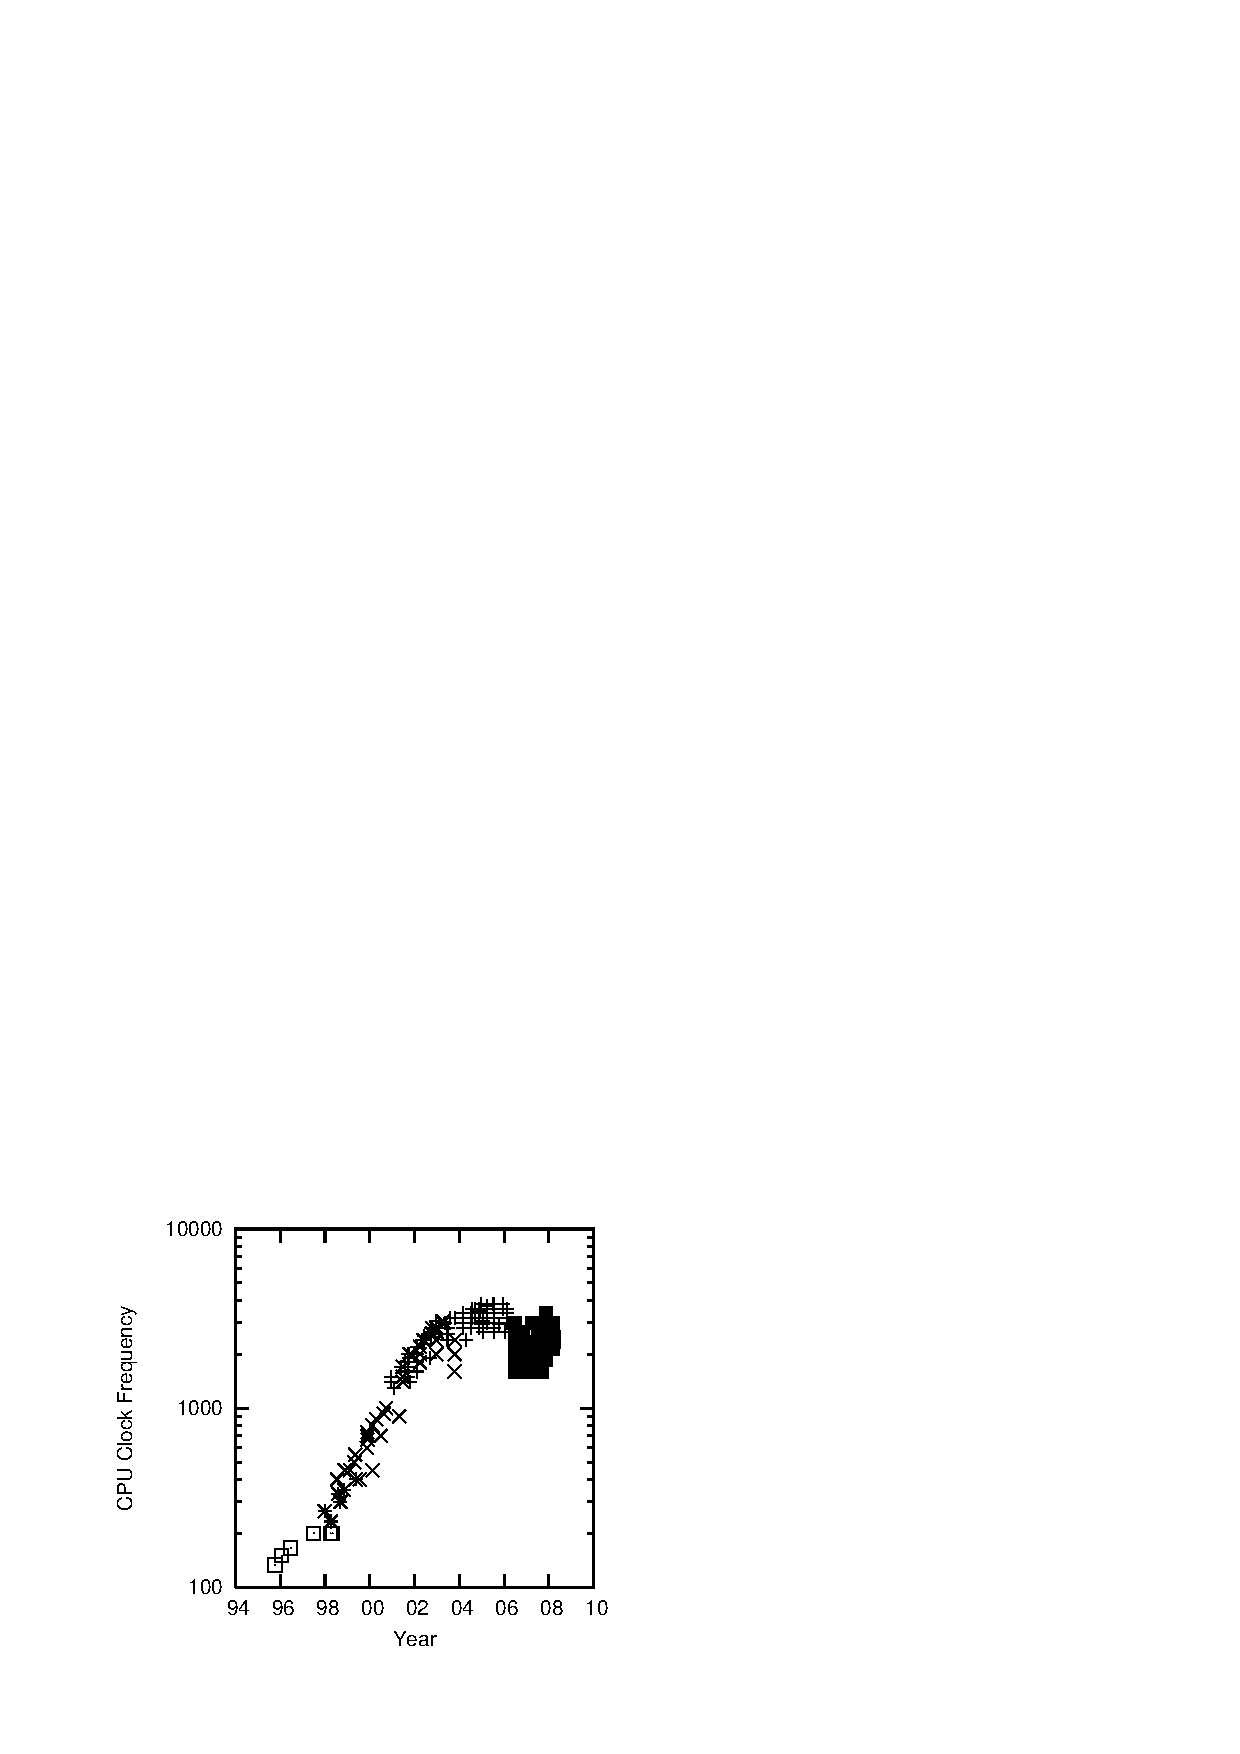
\includegraphics{SMPdesign/clockfreq}}
\end{center}
\caption{MIPS/Clock-Frequency Trend for Intel CPUs}
\label{fig:intro:Clock-Frequency Trend for Intel CPUs}
\end{figure}

That said, the focus of performance has shifted from hardware to
parallel software.
This change in focus is due to the fact that, although Moore's Law
continues to deliver increases in transistor density, it has ceased to
provide the traditional single-threaded performance increases.
This can be seen in
Figure~\ref{fig:intro:Clock-Frequency Trend for Intel CPUs}.\footnote{	
	This plot shows clock frequencies for newer CPUs theoretically
	capable of retiring one or more instructions per clock, and MIPS
	(millions of instructions per second, usually from the old
	Dhrystone benchmark)
	for older CPUs requiring multiple clocks to execute even the
	simplest instruction.
	The reason for shifting between these two measures is that the
	newer CPUs' ability to retire multiple instructions per clock is
	typically limited by memory-system performance.
	Furthermore, the benchmarks commonly used on the older CPUs
	are obsolete, and it is difficult to run the newer benchmarks
	on systems containing the old CPUs, in part because it is hard
	to find working instances of the old CPUs.},
which shows that writing single-threaded code and simply waiting
a year or two for the CPUs to catch up may no longer be an option.
Given the recent trends on the part of all major manufacturers towards
multicore/multithreaded systems, parallelism is the way to go for
those wanting the avail themselves of the full performance of their
systems.

Even so, the first goal is performance rather than scalability,
especially given that the easiest way to attain linear scalability
is to reduce the performance of each CPU~\cite{LinusTorvalds2001a}.
Given a four-CPU system, which would you prefer?
A program that provides 100 transactions per second on a single CPU,
but does not scale at all?
Or a program that provides 10 transactions per second on a single CPU,
but scales perfectly?
The first program seems like a better bet, though the answer might
change if you happened to be one of the lucky few with access to a
32-CPU system.

That said, just because you have multiple CPUs is not necessarily
in and of itself a reason to use them all, especially given the
recent decreases in price of multi-CPU systems.
The key point to understand is that parallel programming is primarily
a performance optimization, and, as such, it is one potential optimization
of many.
If your program is fast enough as currently written, there is no
reason to optimize, either by parallelizing it or by applying any
of a number of potential sequential optimizations.\footnote{
	Of course, if you are a hobbyist whose primary interest is
	writing parallel software, that is more than enough reason to
	parallelize whatever software you are interested in.}
By the same token, if you are looking to apply parallelism as an
optimization to a sequential program, then you will need to compare
parallel algorithms to the best sequential algorithms.
This may require some care, as far too many publications ignore the
sequential case when analyzing the performance of parallel algorithms.

\subsection{Productivity}
\label{sec:intro:Productivity}

\QuickQuiz{}
	Why all this prattling on about non-technical issues???
	And not just \emph{any} non-technical issue, but \emph{productivity}
	of all things?
	Who cares?
\QuickQuizAnswer{
	If you are a pure hobbyist, perhaps you don't need to care.
	But even pure hobbyists will often care about how much they
	can get done, and how quickly.
	After all, the most popular hobbyist tools are usually those
	that are the best suited for the job, and an important part of
	the definition of ``best suited'' involves productivity.
	And if someone is paying you to write parallel code, they will
	very likely care deeply about your productivity.
	And if the person paying you cares about something, you would
	be most wise to pay at least some attention to it!

	Besides, if you \emph{really} didn't care about productivity,
	you would be doing it by hand rather than using a computer!
} \QuickQuizEnd

Productivity has been becoming increasingly important through the decades.
To see this, consider that early computers cost millions of dollars at
a time when engineering salaries were a few thousand dollars a year.
If dedicating a team of ten engineers to such a machine would improve
its performance by 10\%, their salaries would be repaid many times over.

One such machine was the CSIRAC, the oldest still-intact stored-program
computer, put in operation in
1949~\cite{CSIRACMuseumVictoria,CSIRACUniversityMelbourne}.
Given that the machine had but 768 words of RAM, it is safe to say
that the productivity issues that arise in large-scale software projects
were not an issue for this machine.
Because this machine was built before the transistor era, it was constructed
of 2,000 vacuum tubes, ran with a clock frequency of 1kHz,
consumed 30kW of power, and weighed more than three metric tons.

It would be difficult to purchase a machine with this little compute
power roughly sixty years later (2008), with the closest equivalents
being 8-bit embedded microprocessors exemplified by the venerable
Z80~\cite{z80Wikipedia}.
This CPU had 8,500 transistors, and can still be purchased in 2008
for less than \$2 US per unit in 1,000-unit quantities.
In stark contrast to the CSIRAC, software-development costs are
anything but insignificant for the Z80.

\begin{figure}[tb]
\begin{center}
\resizebox{3in}{!}{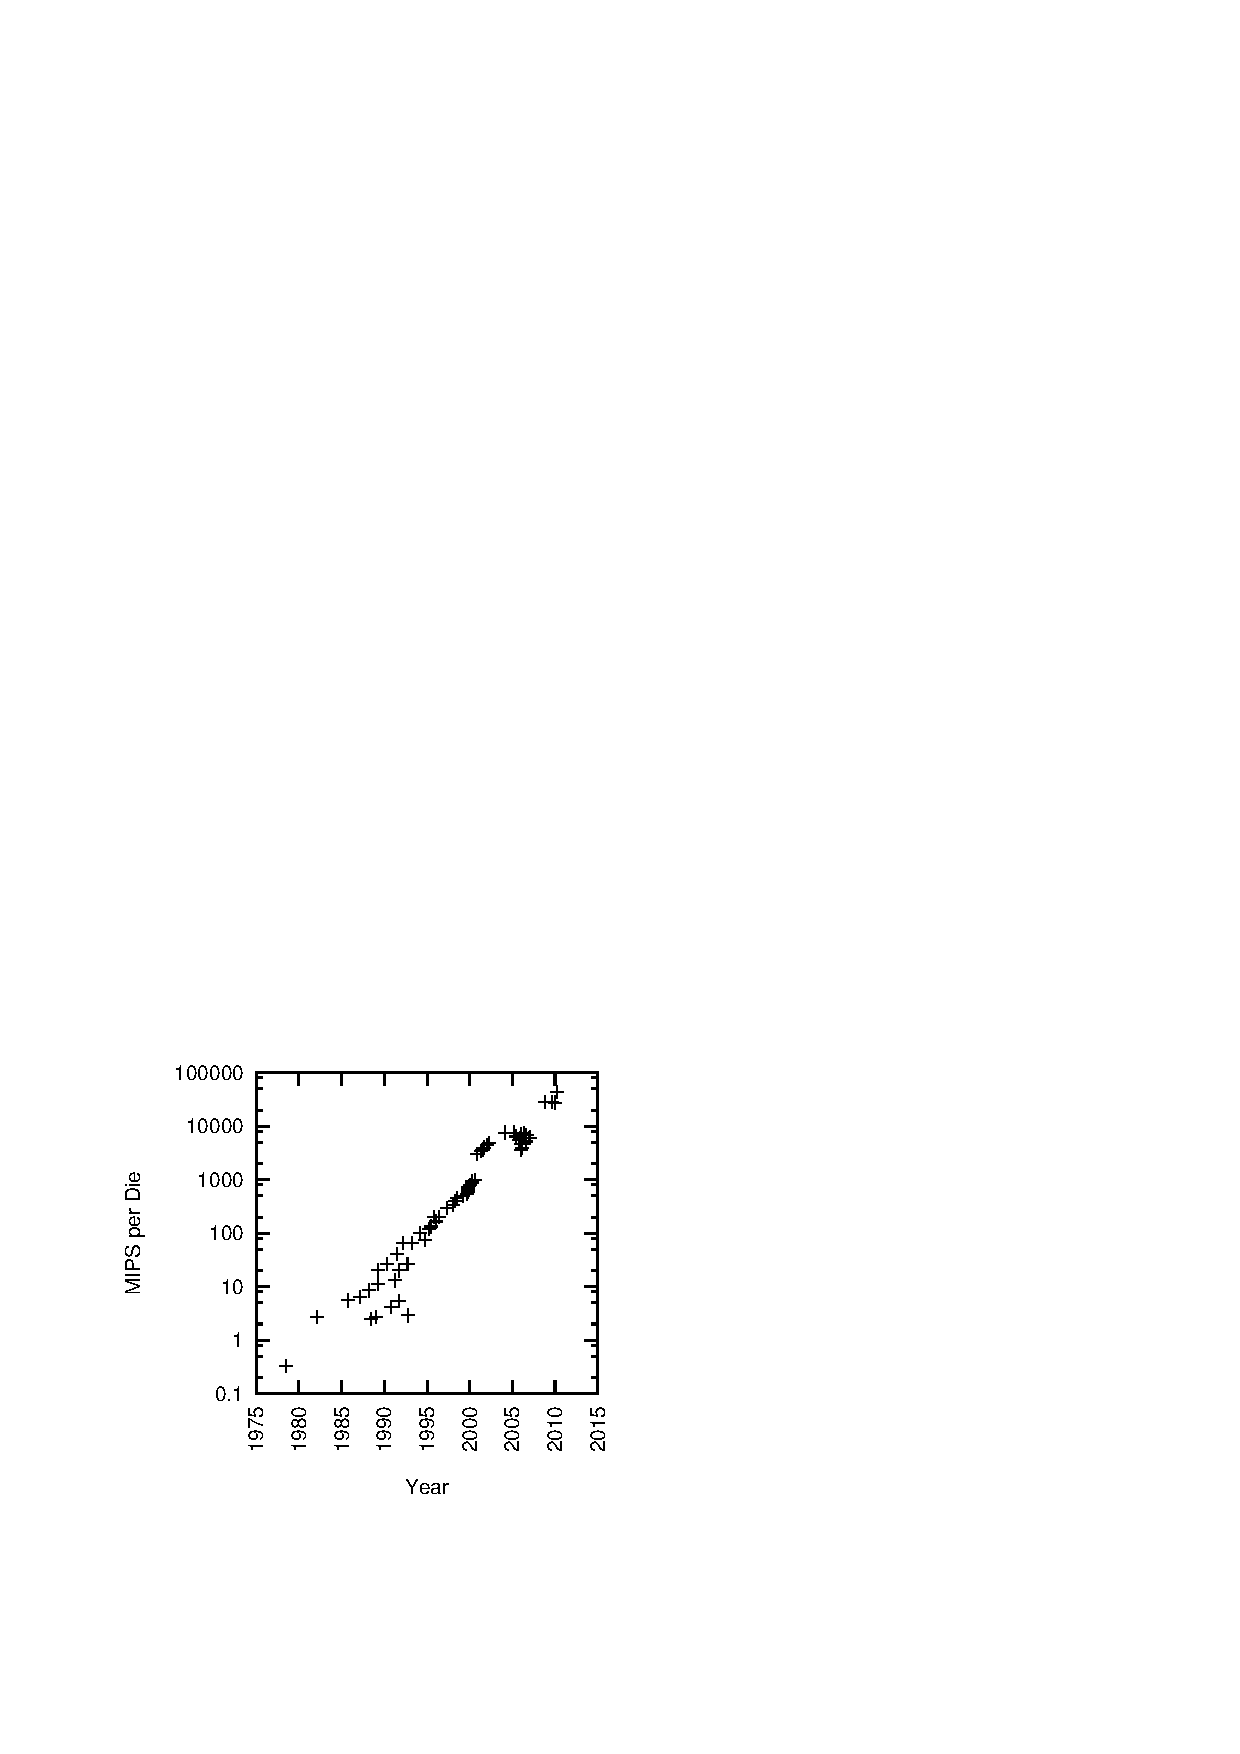
\includegraphics{SMPdesign/mipsperbuck}}
\end{center}
\caption{MIPS per Die for Intel CPUs}
\label{fig:intro:MIPS per Die for Intel CPUs}
\end{figure}

The CSIRAC and the Z80 are two points in a long-term trend, as can be
seen in
Figure~\ref{fig:intro:MIPS per Die for Intel CPUs}.
This figure plots an approximation to computational power per die
over the past three decades, showing a consistent four-order-of-magnitude
increase.
Note that the advent of multicore CPUs has permitted this increase to
continue unabated despite the clock-frequency wall encountered in 2003.

One of the inescapable consequences of the rapid decrease in
the cost of hardware is that software productivity grows increasingly
important.
It is no longer sufficient merely to make efficient use of the hardware,
it is now also necessary to make extremely efficient use of software
developers.
This has long been the case for sequential hardware, but only recently
has parallel hardware become a low-cost commodity.
Therefore, the need for high productivity in creating parallel software
has only recently become hugely important.

\QuickQuiz{}
	Given how cheap parallel hardware has become, how can anyone
	afford to pay people to program it?
\QuickQuizAnswer{
	There are a number of answers to this question:
	\begin{enumerate}
	\item	Given a large computational cluster of parallel machines,
		the aggregate cost of the cluster can easily justify
		substantial developer effort, because the development
		cost can be spread over the large number of machines.
	\item	Popular software that is run by tens of millions of users
		can easily justify substantial developer effort,
		as the cost of this development can be spread over the tens
		of millions of users.
		Note that this includes things like kernels and system
		libraries.
	\item	If the low-cost parallel machine is controlling the operation
		of a valuable piece of equipment, then the cost of this
		piece of equipment might easily justify substantial
		developer effort.
	\item	If the software for the low-cost parallel produces an
		extremely valuable result (e.g., mineral exploration),
		then the valuable result might again justify substantial
		developer cost.
	\item	Safety-critical systems protect lives, which can clearly
		justify very large developer effort.
	\item	Hobbyists and researchers might seek knowledge, experience,
		fun, or glory rather than mere money.
	\end{enumerate}
	So it is not the case that the decreasing cost of hardware renders
	software worthless, but rather that it is no longer possible to
	``hide'' the cost of software development within the cost of
	the hardware, at least not unless there are extremely large
	quantities of hardware.
} \QuickQuizEnd

Perhaps at one time, the sole purpose of parallel software was performance.
Now, however, productivity is increasingly important.

\subsection{Generality}
\label{sec:intro:Generality}

One way to justify the high cost of developing parallel software
is to strive for maximal generality.
All else being equal, the cost of a more-general software artifact
can be spread over more users than can a less-general artifact.

Unfortunately, generality often comes at the cost of performance,
productivity, or both.
To see this, consider the following popular parallel programming
environments:

\begin{description}
\item[C/C++ ``Locking Plus Threads'']: This category, which includes
	POSIX Threads (pthreads)~\cite{OpenGroup1997pthreads},
	Windows Threads, and numerous
	operating-system kernel environments, offers excellent performance
	(at least within the confines of a single SMP system)
	and also offers good generality.
	Pity about the relatively low productivity.
\item[Java]: This programming environment, which is inherently
	multithreaded, is widely believed to be much more productive
	than C or C++, courtesy of the automatic garbage collector
	and the rich set of class libraries, and is reasonably
	general purpose.
	However, its performance, though greatly improved in the early
	2000s, is generally considered to be less than that of C and C++.
\item[MPI]: This Message Passing Interface~\cite{MPIForum2008} powers
	the largest scientific and technical computing clusters in
	the world, so offers unparalleled performance and scalability.
	It is in theory general purpose, but has generally been used
	for scientific and technical computing.
	Its productivity is believed by many to be even lower than that
	of C/C++ ``locking plus threads'' environments.
\item[OpenMP]: This set of compiler directives can be used
	to parallelize loops.  It is thus quite specific to this
	task, and this specificity often limits its performance.
	It is, however, much easier to use than MPI or C/C++
	``locking plus threads.''
\item[SQL]: Structured Query Language~\cite{DIS9075SQL92} is extremely
	specific, applying only to relational database queries.
	However, its performance is quite good, doing quite well
	in Transaction Processing Performance Council (TPC)
	benchmarks~\cite{TPC}.
	Productivity is excellent, in fact, this parallel programming
	environment enables parallel-programming novices
	to make good use of a large parallel system.
\end{description}

\begin{figure}[tb]
\begin{center}
\resizebox{3in}{!}{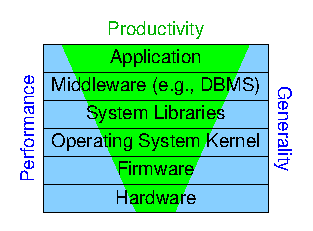
\includegraphics{intro/PPGrelation}}
\end{center}
\caption{Software Layers and Performance, Productivity, and Generality}
\label{fig:intro:Software Layers and Performance, Productivity, and Generality}
\end{figure}

The nirvana of parallel programming environments, one that offers
world-class performance, productivity, and generality, simply does
not yet exist.
Until such a nirvana appears, it will be necessary to make engineering
tradeoffs among performance, productivity, and generality.
One such tradeoff is shown in
Figure~\ref{fig:intro:Software Layers and Performance, Productivity, and Generality},
which shows how productivity becomes increasingly important at the upper layers
of the system stack,
while performance and generality become increasingly important at the
lower layers of the system stack.
The huge development costs incurred near the bottom of the stack
must be spread over equally huge numbers of users on the one hand
(hence the importance of generality), and
performance lost near the bottom of the stack cannot easily be
recovered further up the stack.
Near the top of the stack, there might be very few users for a given
specific application, in which case productivity concerns are paramount.
This explains the tendency towards ``bloatware'' further up the stack:
extra hardware is often cheaper than the extra developers.
This book is intended for developers working near the bottom
of the stack, where performance and generality are of great concern.

\begin{figure}[tb]
\begin{center}
\resizebox{3in}{!}{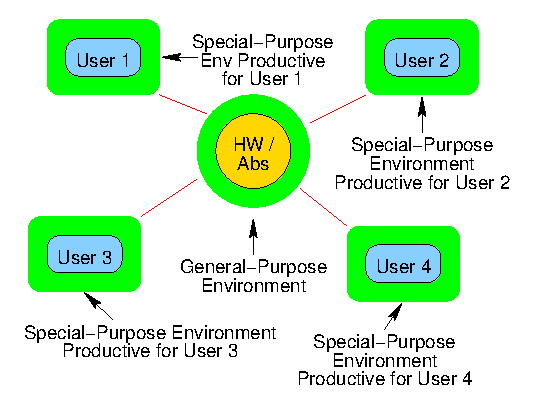
\includegraphics{intro/Generality}}
\end{center}
\caption{Tradeoff Between Productivity and Generality}
\label{fig:intro:Tradeoff Between Productivity and Generality}
\end{figure}

It is important to note that a tradeoff between productivity and
generality has existed for centuries in many fields.
For but one example, a nailgun is far more productive than is a
hammer, but in contrast to the nailgun, a hammer can be used for
many things besides driving nails.
It should therefore be absolutely no surprise to see similar tradeoffs
appear in the field of parallel computing.
This tradeoff is shown schematically in
Figure~\ref{fig:intro:Tradeoff Between Productivity and Generality}.
Here, users~1, 2, 3, and 4 have specific jobs that they need the computer
to help them with.
The most productive possible language or environment for a given user is one
that simply does that user's job, without requiring any programming,
configuration, or other setup.

\QuickQuiz{}
	This is a ridiculously unachievable ideal!
	Why not focus on something that is achievable in practice?
\QuickQuizAnswer{
	This is eminently achievable.
	The cellphone is a computer that can be used to make phone
	calls and to send and receive text messages with little or
	no programming or configuration on the part of the end user.

	This might seem to be a trivial example at first glance,
	but if you consider it carefully you will see that it is
	both simple and profound.
	When we are willing to sacrifice generality, we can achieve
	truly astounding increases in productivity.
	Those who cling to generality will therefore fail to set
	the productivity bar high enough to succeed in production
	environments.
} \QuickQuizEnd

Unfortunately, a system that does the job required by user~1 is
unlikely to do user~2's job.
In other words, the most productive languages and environments are
domain-specific, and thus by definition lacking generality.

Another option is to tailor a given programming language or environment
to the hardware system (for example, low-level languages such as
assembly, C, C++, or Java) or to some abstraction (for example,
Haskell, Prolog, or Snobol), as is shown by the circular region near
the center of
Figure~\ref{fig:intro:Tradeoff Between Productivity and Generality}.
These languages can be considered to be general in the sense that they
are equally ill-suited to the jobs required by users~1, 2, 3, and 4.
In other words, their generality is purchased at the expense of
decreased productivity when compared to domain-specific languages
and environments.
Worse yet, a language that is tailored to a given abstraction
is also likely to suffer from performance and scalability problems
unless and until someone figures out how to efficiently map that
abstraction to real hardware.

With the three often-conflicting parallel-programming goals of
performance, productivity,
and generality in mind, it is now time to look into avoiding these
conflicts by considering alternatives to
parallel programming.

\section{Alternatives to Parallel Programming}
\label{sec:intro:Alternatives to Parallel Programming}

In order to properly consider alternatives to parallel programming,
you must first have thought through what you expect the parallelism
to do for you.
As seen in Section~\ref{sec:intro:Parallel Programming Goals},
the primary goals of parallel programming are performance, productivity,
and generality.
Because this book is intended for developers working on
performance-critical code near the bottom of the software stack,
the remainder of this section focuses primarily on performance improvement.

It is important to keep in mind that parallelism is but one way to
improve performance.
Other well-known approaches include the following, in roughly increasing
order of difficulty:

\begin{enumerate}
\item	Run multiple instances of a sequential application.
\item	Make the application use existing parallel software.
\item	Apply performance optimization to the serial application.
\end{enumerate}

These approaches are covered in the sections.

\subsection{Multiple Instances of a Sequential Application}
\label{sec:intro:Multiple Instances of a Sequential Application}

Running multiple instances of a sequential application can allow you
to do parallel programming without actually doing parallel programming.
There are a large number of ways to approach this, depending on the
structure of the application.

If your program is analyzing a large number of different scenarios,
or is analyzing a large number of independent data sets, one easy
and effective approach is to create a single sequential program that
carries out a single analysis, then use any of a number of scripting
environments (for example the \co{bash} shell) to run a number of
instances of this sequential program in parallel.
In some cases, this approach can be easily extended to a cluster of
machines.

This approach may seem like cheating, and in fact some denigrate such
programs as ``embarrassingly parallel''.
And in fact, this approach does have some potential disadvantages,
including increased memory consumption, waste of CPU cycles recomputing
common intermediate results, and increased copying of data.
However, it is often  extremely productive, garnering extreme performance
gains with little or no added effort.

\subsection{Use Existing Parallel Software}
\label{sec:intro:Use Existing Parallel Software}

There is no longer any shortage of parallel software environments that
can present a single-threaded programming environment,
including relational
databases~\cite{Date82},
web-application servers, and map-reduce environments.
For example, a common design provides a separate program for each
user, each of which generates SQL that is run concurrently against a common
relational database.
The per-user programs are responsible only for the user interface,
with the relational database taking full responsibility for the
difficult issues surrounding parallelism and persistence.

Taking this approach often sacrifices some performance, at least when
compared to carefully hand-coding a fully parallel application.
However, such sacrifice is often justified given the huge reduction in
development effort required.

\subsection{Performance Optimization}
\label{sec:intro:Performance Optimization}

Up through the early 2000s, CPU performance was doubling every 18 months.
In such an environment, it is often much more important to create new
functionality than to do careful performance optimization.
Now that Moore's Law is ``only'' increasing transistor density instead
of increasing both transistor density and per-transistor performance,
it might be a good time to rethink the importance of performance
optimization.
After all, performance optimization can reduce power consumption as
well as increasing performance.

From this viewpoint, parallel programming is but another performance
optimization, albeit one that is becoming much more attractive
as parallel systems become cheaper and more readily available.
However, it is wise to keep in mind that the speedup available from
parallelism is limited to roughly the number of CPUs, while the
speedup potentially available from straight software optimization
can be multiple orders of magnitude.

Furthermore, different programs might have different performance
bottlenecks.
Parallel programming will only help with some bottlenecks.
For example, if your program spends most of its time
waiting on data from your disk drive,
using multiple CPUs is not likely to gain much performance.
In fact, if the program was reading from a large file laid out
sequentially on a rotating disk, parallelizing your program might
well make it a lot slower.
You should instead add more disk drives, optimize the data so that
the file can be smaller (thus faster to read), or, if possible,
avoid the need to read quite so much of the data.

\QuickQuiz{}
	What other bottlenecks might prevent additional CPUs from
	providing additional performance?
\QuickQuizAnswer{
	There are any number of potential bottlenecks:
	\begin{enumerate}
	\item	Main memory.  If a single thread consumes all available
		memory, additional threads will simply page themselves
		silly.
	\item	Cache.  If a single thread's cache footprint completely
		fills any shared CPU cache(s), then adding more threads
		will simply thrash the affected caches.
	\item	Memory bandwidth.  If a single thread consumes all available
		memory bandwidth, additional threads will simply
		result in additional queuing on the system interconnect.
	\item	I/O bandwidth.  If a single thread is I/O bound,
		adding more threads will simply result in them all
		waiting in line for the affected I/O resource.
	\end{enumerate}

	Specific hardware systems might have any number of additional
	bottlenecks.
} \QuickQuizEnd

Parallelism can be a powerful optimization technique, but
it is not the only such technique, nor is it appropriate for all
situations.
Of course, the easier it is to parallelize your program, the
more attractive parallelization becomes as an optimization.
Parallelization has a reputation of being quite difficult,
which leads to the question ``exactly what makes parallel
programming so difficult?''

\section{What Makes Parallel Programming Hard?}
\label{sec:intro:What Makes Parallel Programming Hard?}

\OriginallyPublished{Section}{sec:intro:What Makes Parallel Programming Hard?}{What Makes Parallel Programming Hard?}{a Portland State University Technical Report}{PaulEMcKenney2009ProgrammingHard}

It is important to note that the difficulty of parallel programming
is as much a human-factors issue as it is a set of technical properties of the
parallel programming problem.
This is the case because we need human beings to be able to tell parallel
systems what to do, and this two-way communication between human and
computer is as much a function of the human as it is of the computer.
Therefore, appeals to abstractions or to mathematical analyses will
necessarily be of severely limited utility.

In the Industrial Revolution, the interface between human and machine
was evaluated by human-factor studies, then called time-and-motion
studies.
Although there have been a few human-factor studies examining parallel
programming~\cite{RyanEccles2005HPCSNovice,RyanEccles2006HPCSNoviceNeeds,
LorinHochstein2005SC,DuaneSzafron1994PEMPDS}, these studies have
been extremely narrowly focused, and hence unable to demonstrate any
general results.
Furthermore, given that the normal range of programmer productivity
spans more than an order of magnitude, it is unrealistic to expect
an affordable study to be capable of detecting (say) a 10\% difference
in productivity.
Although the multiple-order-of-magnitude differences that such studies
\emph{can} reliably detect are extremely valuable, the most impressive
improvements tend to be based on a long series of 10\% improvements.

We must therefore take a different approach.

\begin{figure}[tb]
\begin{center}
\resizebox{3in}{!}{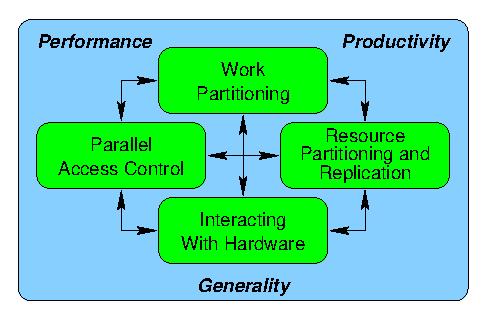
\includegraphics{intro/FourTaskCategories}}
\end{center}
\caption{Categories of Tasks Required of Parallel Programmers}
\label{fig:intro:Categories of Tasks Required of Parallel Programmers}
\end{figure}

One such approach is to carefully consider the tasks that parallel
programmers must undertake that are not required of sequential programmers.
We can then evaluate how well a given programming language or environment
assists the developer with these tasks.
These tasks fall into the four categories shown in
Figure~\ref{fig:intro:Categories of Tasks Required of Parallel Programmers},
each of which is covered in the following sections.

\subsection{Work Partitioning}
\label{sec:intro:Work Partitioning}

Work partitioning is absolutely required for parallel execution:
if there is but one ``glob'' of work, then it can be executed by at
most one CPU at a time, which is by definition sequential execution.
However, partitioning the code requires great care.
For example, uneven partitioning can result in sequential execution
once the small partitions have completed~\cite{GeneAmdahl1967AmdahlsLaw}.
In less extreme cases, load balancing can be used to fully utilize
available hardware, thus improving performance and scalabilty.

In addition, partitioning of work can complicate handling of global
errors and events: a parallel
program may need to carry out non-trivial synchronization in order
to safely process such global events.

Each partition requires some sort of communication: after all, if
a given thread did not communicate at all, it would have no effect and
would thus not need to be executed.
However, because communication incurs overhead, careless partitioning choices
can result in severe performance degradation.

Furthermore, the number of concurrent threads must often be controlled,
as each such thread occupies common resources, for example,
space in CPU caches.
If too many threads are permitted to execute concurrently, the
CPU caches will overflow, resulting in high cache miss rate, which in
turn degrades performance.
On the other hand, large numbers of threads are often required to
overlap computation and I/O.

\QuickQuiz{}
	What besides CPU cache capacity might require limiting the
	number of concurrent threads?
\QuickQuizAnswer{
	There are any number of potential limits on the number of
	threads:
	\begin{enumerate}
	\item	Main memory.  Each thread consumes some memory
		(for its stack if nothing else), so that excessive
		numbers of threads can exhaust memory, resulting
		in excessive paging or memory-allocation failures.
	\item	I/O bandwidth.  If each thread initiates a given
		amount of mass-storage I/O or networking traffic,
		excessive numbers of threads can result in excessive
		I/O queuing delays, again degrading performance.
		Some networking protocols may be subject to timeouts
		or other failures if there are so many threads that
		networking events cannot be responded to in a timely
		fashion.
	\item	Synchronization overhead.
		For many synchronization protocols, excessive numbers
		of threads can result in excessive spinning, blocking,
		or rollbacks, thus degrading performance.
	\end{enumerate}

	Specific applications and platforms may have any number of additional
	limiting factors.
} \QuickQuizEnd

Finally, permitting threads to execute concurrently greatly increases
the program's state space, which can make the program difficult to
understand, degrading productivity.
All else being equal, smaller state spaces having more regular structure
are more easily understood, but this is a human-factors statement as much
as it is a technical or mathematical statement.
Good parallel designs might have extremely large state spaces, but
nevertheless be easy to understand due to their regular structure,
while poor designs can be impenetrable despite having a comparatively
small state space.
The best designs exploit embarrassing parallelism, or transform the
problem to one having an embarrassingly parallel solution.
In either case, ``embarrassingly parallel'' is in fact
an embarrassment of riches.
The current state of the art enumerates good designs; more work is
required to make more general judgments on
state-space size and structure.

\subsection{Parallel Access Control}
\label{sec:Parallel Access Control}

Given a sequential program with only a single thread, that single
thread has full access to all of the program's resources.
These resources are most often in-memory data structures, but can be CPUs,
memory (including caches), I/O devices, computational accelerators, files,
and much else besides.

The first parallel-access-control issue is whether the form of the access to
a given resource depends on that resource's location.
For example, in many message-passing environments, local-variable
access is via expressions and assignments,
while remote-variable access uses an entirely different
syntax, usually involving messaging.
The POSIX Threads environment~\cite{OpenGroup1997pthreads},
Structured Query Language (SQL)~\cite{DIS9075SQL92}, and
partitioned global address-space (PGAS) environments
such as Universal Parallel C (UPC)~\cite{ElGhazawi2003UPC}
offer implicit access,
while Message Passing Interface (MPI)~\cite{MPIForum2008} offers
explicit access because access to remote data requires explicit
messaging.

The other parallel-access-control issue is how threads coordinate
access to the resources.
This coordination is carried out by
the very large number of synchronization mechanisms
provided by various parallel languages and environments,
including message passing, locking, transactions,
reference counting, explicit timing, shared atomic variables, and data
ownership.
Many traditional parallel-programming concerns such as deadlock,
livelock, and transaction rollback stem from this coordination.
This framework can be elaborated to include comparisons
of these synchronization mechanisms, for example locking vs. transactional
memory~\cite{McKenney2007PLOSTM}, but such elaboration is beyond the
scope of this section.

\subsection{Resource Partitioning and Replication}
\label{sec:Resource Partitioning and Replication}

The most effective parallel algorithms and systems exploit resource
parallelism, so much so that it is
usually wise to begin parallelization by partitioning your write-intensive
resources and replicating frequently accessed read-mostly resources.
The resource in question is most frequently data, which might be
partitioned over computer systems, mass-storage devices, NUMA nodes,
CPU cores (or dies or hardware threads), pages, cache lines, instances
of synchronization primitives, or critical sections of code.
For example, partitioning over locking primitives is termed
``data locking''~\cite{Beck85}.

Resource partitioning is frequently application dependent, for
example, numerical applications frequently partition matrices
by row, column, or sub-matrix, while commercial applications frequently
partition write-intensive data structures and replicate
read-mostly data structures.
For example, a commercial application might assign the data for a
given customer to a given few computer systems out of a large cluster.
An application might statically partition data, or dynamically
change the partitioning over time.

Resource partitioning is extremely effective, but
it can be quite challenging for complex multilinked data
structures.

\subsection{Interacting With Hardware}
\label{sec:Interacting With Hardware}

Hardware interaction is normally the domain of the operating system,
the compiler, libraries, or other software-environment infrastructure.
However, developers working with novel hardware features and components
will often need to work directly with such hardware.
In addition, direct access to the hardware can be required when squeezing
the last drop of performance out of a given system.
In this case, the developer may need to tailor or configure the application
to the cache geometry, system topology, or interconnect protocol of the
target hardware.

In some cases, hardware may be considered to be a resource which
may be subject to partitioning or access control, as described in
the previous sections.

\subsection{Composite Capabilities}
\label{sec:Composite Capabilities}

\begin{figure}[tb]
\begin{center}
\resizebox{3in}{!}{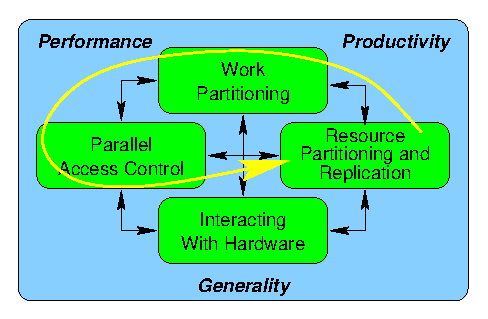
\includegraphics{intro/FourTaskOrder}}
\end{center}
\caption{Ordering of Parallel-Programming Tasks}
\label{fig:intro:Ordering of Parallel-Programming Tasks}
\end{figure}

Although these four capabilities are fundamental,
good engineering practice uses composites of
these capabilities.
For example, the data-parallel approach first
partitions the data so as to minimize the need for
inter-partition communication, partitions the code accordingly,
and finally maps data partitions and threads so as to maximize
throughput while minimizing inter-thread communication,
as shown in
Figure~\ref{fig:intro:Ordering of Parallel-Programming Tasks}.
The developer can then
consider each partition separately, greatly reducing the size
of the relevant state space, in turn increasing productivity.
Of course, some problems are non-partitionable but on the other hand,
clever transformations into forms permitting partitioning can greatly
enhance
both performance and scalability~\cite{PanagiotisMetaxas1999PDCS}.

\subsection{How Do Languages and Environments Assist With These Tasks?}
\label{sec:intro:How Do Languages and Environments Assist With These Tasks?}

Although many environments require that the developer deal manually
with these tasks, there are long-standing environments that bring
significant automation to bear.
The poster child for these environments is SQL, many implementations
of which automatically parallelize single large queries and also
automate concurrent execution of independent queries and updates.

These four categories of tasks must be carried out in all parallel
programs, but that of course does not necessarily mean that the developer
must manually carry out these tasks.
We can expect to see ever-increasing automation of these four tasks
as parallel systems continue to become cheaper and more readily available.

\QuickQuiz{}
	Are there any other obstacles to parallel programming?
\QuickQuizAnswer{
	There are a great many other potential obstacles to parallel
	programming.
	Here are a few of them:
	\begin{enumerate}
	\item	The only known algorithms for a given project might
		be inherently sequential in nature.
		In this case, either avoid parallel programming
		(there being no law saying that your project \emph{has}
		to run in parallel) or invent a new parallel algorithm.
	\item	The project allows binary-only plugins that share the same
		address space, such that no one developer has access to
		all of the source code for the project.
		Because many parallel bugs, including deadlocks, are
		global in nature, such binary-only plugins pose a severe
		challenge to current software development methodologies.
		This might well change, but for the time being, all
		developers of parallel code sharing a given address space
		need to be able to see \emph{all} of the code running in
		that address space.
	\item	The project contains heavily used APIs that were designed
		without regard to
		parallelism~\cite{HagitAttiya2011LawsOfOrder}.
		Some of the more ornate features of the System V
		message-queue API form a case in point.
		Of course, if your project has been around for a few
		decades, and if its developers did not have access to
		parallel hardware, your project undoubtedly has at least
		its share of such APIs.
	\item	The project was implemented without regard to parallelism.
		Given that there are a great many techniques that work
		extremely well in a sequential environment, but that
		fail miserably in parallel environments, if your project
		ran only on sequential hardware for most of its lifetime,
		then your project undoubtably has at least its share of
		parallel-unfriendly code.
	\item	The project was implemented without regard to good
		software-development practice.
		The cruel truth is that shared-memory parallel
		environments are often much less forgiving of sloppy
		development practices than are sequential environments.
		You may be well-served to clean up the existing design
		and code prior to attempting parallelization.
	\item	The people who originally did the development on your
		project have since moved on, and the people remaining,
		while well able to maintain it or add small features,
		are unable to make ``big animal'' changes.
		In this case, unless you can work out a very simple
		way to parallelize your project, you will probably
		be best off leaving it sequential.
		That said, there are a number of simple approaches that
		you might use
		to parallelize your project, including running multiple
		instances of it, using a parallel implementation of
		some heavily used library function, or making use of
		some other parallel project, such as a database.
	\end{enumerate}

	One can argue that many of these obstacles are non-technical
	in nature, but that does not make them any less real.
	In short, parallelization of a large body of code
	can be a large and complex effort.
	As with any large and complex effort, it makes sense to
	do your homework beforehand.
} \QuickQuizEnd

\section{Guide to This Book}
\label{sec:intro:Guide to This Book}

This book is not a collection of optimal algorithms with tiny areas of
applicability; instead, it is a handbook of widely applicable and heavily
used techniques.
We of course could not resist the urge to include some of our favorites
that have not (yet!) passed the test of time (what author could?), but
we have nonetheless gritted our teeth and banished our darlings to
appendices.
Perhaps in time, some of them will see enough use that we can promote
them into the main body of the text.

% \emph{@@@ More here.  Sections.  Layered Approach.  Appendices.
% Glossary.  Bibliography.}

\subsection{Quick Quizzes}

``Quick quizzes'' appear throughout this book.
Some of these quizzes are based on material in which that quick quiz
appears, but others require you to think beyond that section, and,
in some cases, beyond the entire book.
As with most endeavors, what you get out of this book is largely
determined by what you are willing to put into it.
Therefore, readers who invest some time into these quizzes will
find their effort repaid handsomely with increased understanding
of parallel programming.

Answers to the quizzes may be found
in
Appendix~\ref{chp:Answers to Quick Quizzes} starting on
page~\pageref{chp:Answers to Quick Quizzes}.

\QuickQuiz{}
	Where are the answers to the Quick Quizzes found?
\QuickQuizAnswer{
	In Appendix~\ref{chp:Answers to Quick Quizzes} starting on
	page~\pageref{chp:Answers to Quick Quizzes}.

	Hey, I thought I owed you an easy one!
} \QuickQuizEnd

\QuickQuiz{}
	Some of the Quick Quiz questions seem to be from the viewpoint
	of the reader rather than the author.
	Is that really the intent?
\QuickQuizAnswer{
	Indeed it is!
	Many are questions that Paul E. McKenney would probably have
	asked if he was a novice student in a class covering this material.
	It is worth noting that Paul was taught most of this material by
	parallel hardware and software, not by professors.
	In Paul's experience, professors are much more likely to provide
	answers to verbal questions than are parallel systems,
	Watson notwithstanding.
	Of course, we could have a lengthy debate over which of professors
	or parallel systems provide the most useful answers to these sorts
	of questions,
	but for the time being let's just agree that usefulness of
	answers varies widely across the population both of professors
	and of parallel systems.

	Other quizzes are quite similar to actual questions that have been
	asked during conference presentations and lectures covering the
	material in this book.
	A few others are from the viewpoint of the author.
} \QuickQuizEnd

\QuickQuiz{}
	These Quick Quizzes just are not my cup of tea.
	What do you recommend?
\QuickQuizAnswer{
	There are a number of alternatives available to you:
	\begin{enumerate}
	\item	Just ignore the Quick Quizzes and read the rest of
		the book.
		You might miss out on the interesting material in
		some of the Quick Quizzes, but the rest of the book
		has lots of good material as well.
		This is an eminently reasonable approach if your main
		goal is to gain a general understanding of the material
		or if you are skimming through to book to find a
		solution to a specific problem.
	\item	If you find the Quick Quizzes distracting but impossible
		to ignore, you can always clone the \LaTeX{} source for
		this book from the git archive.
		Then modify \co{Makefile} and \co{qqz.sty} to eliminate
		the Quick Quizzes from the PDF output.
		Alternatively, you could modify these two files so as
		to pull the answers inline, immediately following
		the questions.
	\item	Look at the answer immediately rather than investing
		a large amount of time in coming up with your own
		answer.
		This approach is reasonable when a given Quick Quiz's
		answer holds the key to a specific problem you are
		trying to solve.
		This approach is also reasonable if you want a somewhat
		deeper understanding of the material, but when you do not
		expect to be called upon to generate parallel solutions given
		only a blank sheet of paper.
	\item	If you prefer a more academic and rigorous treatment of
		parallel programming,
		you might like Herlihy's and Shavit's
		textbook~\cite{HerlihyShavit2008Textbook}.
		This book starts with an interesting combination
		of low-level primitives at high levels of abstraction
		from the hardware, and works its way through locking
		and simple data structures including lists, queues,
		hash tables, and counters, culminating with transactional
		memory.
		Michael Scott's textbook~\cite{MichaelScott2013Textbook}
		approaches similar material with more of a
		software-engineering focus, and as far as I know, is
		the first formally published textbook to include a
		section devoted to RCU.
	\item	If you would like an academic treatment of parallel
		programming from a programming-language-pragmatics viewpoint,
		you might be interested in the concurrency chapter from Scott's
		textbook~\cite{MichaelScott2006Textbook}
		on programming languages.
	\item	If you are interested in an object-oriented patternist
		treatment of parallel programming focussing on C++,
		you might try Volumes~2 and 4 of Schmidt's POSA
		series~\cite{SchmidtStalRohnertBuschmann2000v2Textbook,
		BuschmannHenneySchmidt2007v4Textbook}.
		Volume 4 in particular has some interesting chapters
		applying this work to a warehouse application.
		The realism of this example is attested to by
		the section entitled ``Partitioning the Big Ball of Mud'',
		wherein the problems inherent in parallelism often
		take a back seat to the problems inherent in getting
		one's head around a real-world application.
	\item	If your primary focus is scientific and technical computing,
		and you prefer a patternist approach,
		you might try Mattson et al.'s
		textbook~\cite{Mattson2005Textbook}.
		It covers Java, C/C++, OpenMP, and MPI.
		Its patterns are admirably focused first on design,
		then on implementation.
	\item	If your primary focus is scientific and technical computing,
		and you are interested in GPUs, CUDA, and MPI, you
		might check out Norm Matloff's ``Programming on
		Parallel Machines''~\cite{NormMatloff2013ParProcBook}.
	\item	If you are interested in POSIX Threads, you might take
		a look at David R. Butenhof's book~\cite{Butenhof1997pthreads}.
	\item	If you are interested in C++11, you might like
		Anthony Williams's ``C++ Concurrency in Action: Practical
		Multithreading''~\cite{AnthonyWilliams2012}.
	\item	If you are interested in C++, but in a Windows environment,
		you might try Herb Sutter's ``Effective Concurrency''
		series in
		Dr. Dobbs Journal~\cite{HerbSutter2008EffectiveConcurrency}.
		This series does a reasonable job of presenting a
		commonsense approach to parallelism.
	\item	If you want to try out Intel Threading Building Blocks,
		then perhaps James Reinders's book~\cite{Reinders2007Textbook}
		is what you are looking for.
	\item	Finally, those preferring to work in Java might be
		well-served by Doug Lea's
		textbooks~\cite{DougLea1997Textbook,Goetz2007Textbook}.
	\end{enumerate}
	In contrast, this book meshes real-world machines with real-world
	algorithms.
	If your sole goal is to find (say) an optimal parallel queue, you
	might be better served by one of the above books.
	However, if you are interested in principles of parallel design
	that allow multiple such queues to operate in parallel, read on!

	Coming back to the topic of Quick Quizzes, if you need a deep
	understanding of the material, then you might well need to
	learn to tolerate the Quick Quizzes.
	Don't get me wrong, passively reading the material can be quite
	valuable, but gaining full problem-solving capability really
	does require that you practice solving problems.

	I learned this the hard way during coursework for my late-in-life
	Ph.D.
	I was studying a familiar topic, and was surprised at how few of
	the chapter's exercises I could solve off the top of my head.
	Forcing myself to answer the questions greatly increased my
	retention of the material.
	So with these Quick Quizzes I am not asking you to do anything
	that I have not been doing myself!
} \QuickQuizEnd

\subsection{Sample Source Code}

This book discusses its fair share of source code, and in many cases
this source code may be found in the \co{CodeSamples} directory
of this book's git tree.
For example, on UNIX systems, you should be able to type:
{\scriptsize
\begin{verbatim}
	find CodeSamples -name rcu_rcpls.c -print
\end{verbatim}
}
to locate the file \co{rcu_rcpls.c}, which is called out in
Section~\ref{sec:defer:``Toy'' RCU Implementations}.
Other types of systems have well-known ways of locating files by
filename.

\begin{figure*}[tbp]
{
\scriptsize
\begin{verbatim}
  1 git clone git://git.kernel.org/pub/scm/linux/kernel/git/paulmck/perfbook.git
  2 cd perfbook
  3 make
  4 evince perfbook.pdf
\end{verbatim}
}
\caption{Creating an Up-To-Date PDF}
\label{fig:intro:Creating a Up-To-Date PDF}
\end{figure*}

\begin{figure*}[tbp]
{
\scriptsize
\begin{verbatim}
  1 git remote update
  2 git checkout origin/master
  3 make
  4 evince perfbook.pdf
\end{verbatim}
}
\caption{Generating an Updated PDF}
\label{fig:intro:Generating an Updated PDF}
\end{figure*}

The source to this book may be found in the \co{git} archive at
\url{git://git.kernel.org/pub/scm/linux/kernel/git/paulmck/perfbook.git},
and \co{git} itself is available as part of most mainstream Linux
distributions.
To create and display a current \LaTeX{} source tree of this book,
use the list of Linux commands shown in
Figure~\ref{fig:intro:Creating a Up-To-Date PDF}.
In some environments, the \co{evince} that displays \co{perfbook.pdf}
may need to be replaced, for example, with \co{acroread}.
The \co{git clone} command need only be used the first time you
create a PDF, subsequently, you can run the commands shown in
Figure~\ref{fig:intro:Generating an Updated PDF} to pull in any updates
and generate an updated PDF.
The commands in
Figure~\ref{fig:intro:Generating an Updated PDF}
must be run within the \co{perfbook} directory created by the commands
shown in
Figure~\ref{fig:intro:Creating a Up-To-Date PDF}.

PDFs of this book are sporadically posted at
\url{http://kernel.org/pub/linux/kernel/people/paulmck/perfbook/perfbook.html}
and at
\url{http://www.rdrop.com/users/paulmck/perfbook/}.
